% Complete Section 5.1, source PDF 61-64 / printed 51-54, including footnote 3 and both figures.
% block: primal-galerkin-heading page:61 type:section
\subsection{{Galerkin discretization of the primal formulation}}\label{sec:primal-galerkin}

% block: primal-galerkin-deficiencies pages:61,62 type:ordinary-paragraph
{A simple approach to discretization of the Hodge Laplacian would be the application of Galerkin's method to the primal weak formulation \eqref{eq:hodge-primal-formulation}, i.e., restricting the trial and test functions to some finite dimensional subspace $V_h\subset V^k\cap V_k^*\cap\mathsf H^{k\perp}$. However, this approach suffers from two serious deficiencies, as we shall now show. First, we can anticipate some difficulty working with the condition $V_h\perp\mathsf H^k$, since in many problems, we do not know the space $\mathsf H^k$ explicitly and may not even know its dimension. We will return to this issue in a moment. Second, \emph{the primal approach may have difficulties even when there are no nonvanishing harmonic forms}. The difficulty here is that the space $V^k\cap V_k^*$ is not a standard Sobolev space, and it may be difficult to design a finite element subspace of it with good approximation properties. More precisely, the space may contain vector fields which are too singular to belong to $H^1$ or even to be approximated arbitrarily closely by $H^1$ vector fields. Such singular fields arise as solutions of the Hodge Laplacian on domains with nonconvex corners and in other situations, so this is a serious defect.}

% block: primal-galerkin-polygon page:62 type:ordinary-paragraph
{As a simple example, suppose that $\Omega$ is a nonconvex simply connected polygon in the plane and consider the two-dimensional $L^2$ de Rham complex, for which the domain complex is}
\[
0\to H^1(\Omega)\xrightarrow{\operatorname{grad}}H(\operatorname{curl},\Omega)\xrightarrow{\operatorname{curl}}L^2(\Omega)\to0
\]
{(here $\operatorname{curl}u=\partial u_2/\partial x_1-\partial u_1/\partial x_2$). Since the domain is simply connected there are no harmonic $1$-forms, and so the primal weak formulation \eqref{eq:hodge-r3-magnetic-primal} of the $k=1$ Hodge Laplacian for this complex seeks $u\in Y:=H(\operatorname{curl})\cap\mathring H(\operatorname{div})$ such that}
\begin{equation}\label{eq:primal-galerkin-polygon}
\int_\Omega[(\operatorname{curl}u)(\operatorname{curl}v)+(\operatorname{div}u)(\operatorname{div}v)]\,dx=\int_\Omega f\cdot v\,dx,\qquad v\in Y.
\end{equation}

% block: primal-galerkin-normal-space page:62 type:ordinary-paragraph
\begingroup\emergencystretch=1em
{Let $H_n^1=H^1(\Omega;\mathbb R^2)\cap\mathring H(\operatorname{div})$ denote the space of $H^1$ vector fields with vanishing normal component on the boundary, which is a closed subspace of $H^1(\Omega;\mathbb R^2)$. Clearly $H_n^1\subset Y$. Moreover,}%
% block: polygon-vector-identity-footnote page:62 type:footnote
\footnote{{This identity follows from a more general one:}
\[
\begin{aligned}
&\int\operatorname{curl}u\operatorname{curl}v\,dx+\int\operatorname{div}u\operatorname{div}v\,dx\\
&\quad=\int\operatorname{grad}u:\operatorname{grad}v\,dx+\sum_e\int_e\left(\frac{\partial u\cdot s}{\partial s}v\cdot n-\frac{\partial u\cdot n}{\partial s}v\cdot s\right)\,ds,\qquad u,v\in H^1(\Omega;\mathbb R^2);
\end{aligned}
\]
{where the sum is over all the edges $e$ of the polygon $\Omega$ and $n$ and $s$ are the (constant) normal and tangent vectors on $e$. This is elementary for $u,v\in C^1(\bar\Omega;\mathbb R^2)$ (integration by parts). Each of the integrals appearing is a bilinear form of $u$ and $v$ bounded with respect to the $H^1$ norm, so we can extend by density. For example,}
\[
\begin{aligned}
\left|\int_e\frac{\partial u\cdot s}{\partial s}v\cdot n\right|&\leq\left\|\frac{\partial u\cdot s}{\partial s}\right\|_{H^{-1/2}(e)}\|v\cdot n\|_{H^{1/2}(e)}\\
&\leq\|u\cdot s\|_{H^{1/2}(e)}\|v\cdot n\|_{H^{1/2}(e)}\leq\|u\|_{H^1(\Omega)}\|v\|_{H^1(\Omega)}.
\end{aligned}
\]
}%
% block: polygon-vector-norm-identity page:62 type:equation
\[
\|\operatorname{curl}u\|^2+\|\operatorname{div}u\|^2=\|\operatorname{grad}u\|^2,\qquad u\in H_n^1.
\]
\par\endgroup

% block: primal-galerkin-closed-proper-subspace page:62 type:ordinary-paragraph
{It follows that the restriction of the $Y$ norm (the norm of $H(\operatorname{div})\cap H(\operatorname{curl})$) to $H_n^1$ is equivalent to the full $H^1$ norm there. Since $H_n^1$ is closed in $H^1$, it is a \emph{closed} subspace of $Y$. Moreover, $H_n^1\ne Y$. This follows from the fact that a generic solution of the Neumann problem for Poisson's equation on a nonconvex polygon exhibits singular behavior near the reentrant corners, which precludes it belonging to $H^2$. Thus there exists $\phi\in H^1(\Omega)$ such that $\Delta\phi\in L^2(\Omega)$ and $\partial\phi/\partial n=0$ on $\partial\Omega$, but $\phi\notin H^2(\Omega)$. Setting $u=\operatorname{grad}\phi$ we see that $u\in Y$ but $u\notin H^1$.}

% block: primal-galerkin-nonapproximation pages:62,63 type:ordinary-paragraph
{In fact, this lack of $H^1$ regularity is typical of solutions of \eqref{eq:primal-galerkin-polygon}. For any such solution, we have $\inf_{v\in H_n^1}\|u-v\|_Y=\delta_u>0$, where $\delta_u$ is the distance of $u$ from the proper closed subspace $H_n^1$. This tells us that if the subspaces $V_h$ are contained in $H_n^1$, then the numerical solution $u_h\in V_h$ cannot converge to $u$. This is the case when $V_h$ is any subspace of $Y$ which consists of piecewise polynomials with respect to some triangulation. Indeed, the condition $V_h\subset H(\operatorname{curl})$ implies that the tangential components of any $v\in V_h$ must be continuous across triangle boundaries, and the fact that $V_h\subset H(\operatorname{div})$ implies that the normal components must be continuous. Thus $V_h$ consists of continuous piecewise polynomial functions, and so $V_h\subset H_n^1$.}

% block: primal-galerkin-l-shaped-figure page:63 type:figure
\begin{figure}[htbp]\centering
\includegraphics[page=63,trim=95bp 507bp 57bp 62bp,clip,width=.96\linewidth]{../input/source/Finite Element Exterior Calculus.pdf}
\caption{{Finite element solution to the Hodge Laplacian problem on an L-shaped domain (with $f=(1,0)$). The left figure is calculated with a mixed method which is known to converge to the solution in $L^2$. The right figure is based on the primal formulation using $24{,}576$ piecewise linear elements. The primal-based numerical solution entirely misses the dominant behavior at the reentrant corner and produces a wholly inaccurate solution.}}\label{fig:primal-lagrange-failure}
\end{figure}

% block: primal-galerkin-nightmare page:63 type:ordinary-paragraph
{In short, \emph{a standard finite element method based on the primal formulation does not generally converge to the solution $u$}. This behavior is illustrated in Figure~\ref{fig:primal-lagrange-failure}, which depicts a numerical analyst's nightmare. The figure on the right shows the numerical solution computed with what would seem to be a natural discretization: the finite element method based on the primal weak formulation, using continuous piecewise linear vector fields as trial functions. The method converges, as the mesh is refined, to what might be taken to be the solution but is, in fact, an altogether different vector field. In three dimensions, the situation is similar but worse, because then $H_n^1$ is a closed subspace of infinite codimension. See \BookCite{34} for an illuminating discussion.}

% block: primal-galerkin-earlier-eigenvalues page:63 type:ordinary-paragraph
{We encountered this problem already in Chapter~\ref{chap:introduction} when we computed the eigenvalues of the vector Laplacian on a polygonal domain with a hole. Because of the reentrant corners, the true eigenfunctions are singular, and the standard finite element method cannot compute them accurately. This results in nonconvergence of the eigenvalues as well, as we saw in the example.}

% block: primal-galerkin-harmonic-loss page:63 type:ordinary-paragraph
{An independent difficulty with the primal formulation arises when there are harmonic forms. The difficulty is that we usually cannot arrange that the harmonic forms belong to the subspace $V_h$. The harmonic forms will generally be smooth functions, but not polynomials. Therefore, if the space $V_h$ is a finite element space, consisting of piecewise polynomials, it will not contain the any nonzero harmonic forms. The discrete problem, to find $u_h\in V_h$ such that}
\[
\langle du_h,dv\rangle+\langle d^*u_h,d^*v\rangle=\langle f,v\rangle,\qquad v\in V_h,
\]
{therefore has a unique solution (the bilinear form on the left-hand side defines an operator $V_h\to V_h'$ with zero kernel). Stated in other terms, the space of discrete harmonic forms vanishes. Therefore, the side condition $u\perp\mathsf H$ is lost on passage to the discrete level. The result, illustrated in Figure~\ref{fig:primal-harmonic-failure}, is that the discrete solution does not resemble the exact solution, even in order of magnitude. Another nightmare!}

% block: primal-galerkin-annulus-figure page:64 type:figure
\begin{figure}[htbp]\centering
\includegraphics[page=64,trim=96bp 513bp 63bp 62bp,clip,width=.96\linewidth]{../input/source/Finite Element Exterior Calculus.pdf}
\caption{{Approximation of the Hodge Laplacian problem on an annulus ($f=(0,x)$). The true solution shown here on the left is an (accurate) approximation by a mixed method. The standard Galerkin solution using continuous piecewise linear vector fields, shown on the right, is totally different.}}\label{fig:primal-harmonic-failure}
\end{figure}
